% Grounded Transport: A Proof-Relevant Rewriting Calculus for Lineage-Sensitive Systems
% FIRST DRAFT.  Build: make   (or: latexmk -pdf paper.tex)
\documentclass[11pt,a4paper]{article}

\usepackage[T1]{fontenc}
\usepackage[utf8]{inputenc}
\usepackage{lmodern}
\usepackage[margin=2.6cm]{geometry}
\usepackage{amsmath,amssymb,amsthm,mathtools,centernot}
\usepackage{booktabs,array,tabularx,longtable}
\usepackage{enumitem}
\usepackage{listings}
\usepackage{tikz}
\usetikzlibrary{arrows.meta,positioning,shapes.geometric}
\usepackage[numbers,sort&compress]{natbib}
\usepackage[hidelinks]{hyperref}
\usepackage{xurl}
\usepackage[capitalise,noabbrev]{cleveref}

\emergencystretch=3em
\setlist{itemsep=2pt,topsep=4pt}

% ---------- theorem environments ----------
\theoremstyle{plain}
\newtheorem{theorem}{Theorem}
\newtheorem{proposition}[theorem]{Proposition}
\newtheorem{lemma}[theorem]{Lemma}
\newtheorem{corollary}[theorem]{Corollary}
\theoremstyle{definition}
\newtheorem{definition}{Definition}
\newtheorem{example}{Example}
\theoremstyle{remark}
\newtheorem{remark}{Remark}

% ---------- macros ----------
\DeclareUrlCommand\coq{\def\UrlFont{\ttfamily\small\upshape}}   % Coq identifiers (breakable)
\newcommand{\GTrans}{\mathsf{GTrans}}
\newcommand{\Cross}{\mathsf{Cross}}
\newcommand{\erase}{\mathsf{erase}}
\newcommand{\src}{\mathsf{src}}
\newcommand{\dst}{\mathsf{dst}}
\newcommand{\Prop}{\mathsf{Prop}}
\newcommand{\Type}{\mathsf{Type}}
\newcommand{\back}{\mathrm{back}}
\newcommand{\fwd}{\mathrm{fwd}}
\newcommand{\Cert}{\mathsf{Certified}}
\newcommand{\Refu}{\mathsf{Refuted}}
\newcommand{\Open}{\mathsf{Open}}
\newcommand{\Assess}{\mathsf{Assessment}}
\newcommand{\Proper}{\mathsf{Proper}}
\newcommand{\GProper}{\mathsf{GroundedProper}}
\newcommand{\anc}{\mathrm{anc}}
\newcommand{\nat}{\mathbb{N}}
\newcommand{\bool}{\mathbb{B}}
\newcolumntype{Y}{>{\raggedright\arraybackslash}X}
\newcommand{\weq}{\mathrel{\simeq}}

\lstset{basicstyle=\ttfamily\footnotesize,columns=fullflexible,keepspaces=true,
        xleftmargin=1em,aboveskip=6pt,belowskip=6pt,breaklines=true,showstringspaces=false}

\title{Grounded Transport:\\ A Proof-Relevant Rewriting Calculus\\ for Lineage-Sensitive Systems}
\author{Author names withheld for review}
\date{\textit{First draft, \today}}

\begin{document}
\maketitle

\begin{abstract}
Ordinary rewriting records that one expression may replace another under an extensional relation.
In lineage-sensitive systems this is not always enough: whether a substitution is warranted may also depend on the process that connects the terms, whether that process was independently grounded, whether its evidence has been maintained through time, and which obligations remain unresolved.
We introduce a directed, proof-relevant transport calculus in which this warrant is carried as extractable data.
Erasure, in two stages, recovers ordinary substitutability; we prove that erasure is sound, that it does not reflect grounding, and that distinct warrants can erase to the same judgement.
Grounded-proper contexts transport witnesses compositionally.
Instantiated on grounded seams, the calculus recovers an earlier seam-transport theorem, separates structural naturality from preservation of grounding, and yields located obstructions to substitution.
Assessment is problem-indexed and three-valued (certified, refuted, open), retains every located failure, and does not treat missing evidence as refutation.
A finite lineage audit is proved to reflect its specification.
The development is mechanised in Coq without axioms in its kernel, and extraction to OCaml shows that certificates, lineage graphs and obstructions survive proof erasure.
The calculus does not establish that declared records are complete or accurate; it makes precisely explicit what is being declared.
\end{abstract}

\section{Introduction}\label{sec:intro}

\subsection{The limitation of extensional rewriting}
Ordinary rewriting licenses substitution under a relation. If $x \mathrel{R} y$ and $C$ is a context that respects the relevant relations, then $C[x] \mathrel{R'} C[y]$. This is deliberately extensional: once $x \mathrel{R} y$ has been established, the rewriting step normally does not retain how $x$ and $y$ were connected, which process produced the claimed agreement, whether one side was copied from the other, whether the evidence was independently grounded, whether the transformation has been maintained through time, or whether any obligation remains open.

For mathematical equality this forgetting is harmless, and it is the source of rewriting's power. For audited migrations, provenance-sensitive predicates, certified transformations and socio-technical assurance it is not always harmless. There, whether a substitution is \emph{warranted} can depend on exactly the information that a relational proof discards.

\subsection{The motivating phenomenon}
Consider a dual-write migration in which two services record a status for each request, and a third source, an execution trace, records what actually happened. On an ordinary request all three agree. On one exceptional request both services report success---because one copied the other---while the trace records failure. The two service records agree with each other, so ordinary relational rewriting between them succeeds; they disagree with the independently exhibited process. If we repair the disagreement by defining the trace valuation to be the first service's value, all equations hold, but the ``ground'' now descends from the coordinate it was supposed to ground. The endpoint equation is true; its evidential warrant has failed.
\Cref{sec:example} works this example out completely; it is the separating model for most of the paper.

\subsection{The proposed solution}
We introduce \emph{grounded transport}, written schematically $\GTrans_c(x,y) : \Type$ for a declared transport problem $c$. An inhabitant is not merely a proof that $x$ and $y$ are related: it carries the evidence by which transport is licensed. Erasure recovers ordinary substitutability in two stages,
\[
\GTrans_c(x,y) \;\xrightarrow{\ \erase_1\ }\; \Cross_c(x,y) \;\xrightarrow{\ \erase_2\ }\; R(x,y),
\]
first forgetting certificates while keeping the directed crossing, then forgetting the crossing while keeping the relation. The central asymmetry is
\[
\GTrans_c(x,y) \Longrightarrow R(x,y), \qquad\text{but in general}\qquad R(x,y) \centernot\Longrightarrow \GTrans_c(x,y).
\]
Ordinary rewriting is therefore the extensional image of the calculus, not something the calculus abandons.

\subsection{Contributions}
\begin{enumerate}
\item \textbf{A grounded transport calculus} (\cref{sec:calculus}). A directed, proof-relevant transport judgement carrying extractable seam, exhibition, lineage, coverage and record evidence, with identity and composition, and with the algebraic laws stated modulo an explicit witness equivalence.
\item \textbf{Erasure theory} (\cref{sec:erasure}). A two-stage erasure, its soundness, the induced preorder, a precise distinction between sound refinement and exact recovery, a proof that erasure does not reflect grounding, and a proof that distinct warrants can erase to the same judgement.
\item \textbf{Contextual preservation} (\cref{sec:contexts}). A $\GProper$ interface for contexts that transport witnesses compositionally, inducing ordinary $\Proper$ instances after erasure.
\item \textbf{Seam and temporal instances} (\cref{sec:seams,sec:dynamic}). A compatibility result recovering an earlier grounded-seam theorem, and a separation of structural naturality, valuation naturality, preservation of grounding, and coverage.
\item \textbf{Obstruction theory} (\cref{sec:obstruction}). Located evidence showing why extensional or observational agreement can fail to warrant lineage-sensitive substitution.
\item \textbf{Evidence-bearing assessment} (\cref{sec:assessment,sec:lineage}). A problem-indexed, three-valued semantics (certified, refuted, open) that retains every located failure, distinguishes missing evidence from counterevidence, and includes a lineage audit proved to reflect its specification.
\item \textbf{Mechanised validation} (\cref{sec:mechanisation}). A Coq development, axiom-free in its kernel and checked with \texttt{coqchk}, with extracted OCaml programs showing that evidential data survive proof erasure.
\end{enumerate}
We do not claim that equality, setoid rewriting, factorisation, or proof-relevant relations are new. The contribution is their integration into one calculus with the properties above.

\subsection{Scope and non-claims}
The calculus does \emph{not} prove that a declared lineage graph is complete; that raw evidence is accurate; that a state model adequately represents a concrete process; that an institutional authority is legitimate or competent; that every transport obligation is decidable; or that ordinary rewriting is unsound. The claim is narrower: ordinary rewriting is \emph{evidentially incomplete} for some applications, and this incompleteness can be repaired without giving up its extensional image. The calculus makes explicit what is declared; it does not make declarations true.

\section{A minimal failure of extensional warrant}\label{sec:example}

This section presents the motivating counterexample in full, before any general definitions. It is the model reused in \cref{sec:erasure,sec:seams,sec:evaluation}.

\subsection{The dual-write span}
Let $\Sigma = \{r_{\mathrm{ok}}, r_*\}$ be a set of requests and take $A = B = \Sigma$, with projections
\[
A \xleftarrow{\ \back\ } \Sigma \xrightarrow{\ \fwd\ } B, \qquad \back = \fwd = \mathrm{id}.
\]
Let both coordinate predicates be constantly true:
\[
\Phi_A(\back(r)) = 1, \qquad \Phi_B(\fwd(r)) = 1 \qquad (r \in \Sigma).
\]
Then $\Phi_A \circ \back = \Phi_B \circ \fwd$: pairwise, extensional seam coherence holds.

\subsection{The independently grounded valuation}
Let the seam carry its own valuation, exhibited from the execution trace:
\[
\Phi_\Sigma(r_{\mathrm{ok}}) = 1, \qquad \Phi_\Sigma(r_*) = 0.
\]
At $r_*$ we have $\Phi_A(\back(r_*)) = \Phi_B(\fwd(r_*)) = 1$ but $\Phi_\Sigma(r_*) = 0$: the coordinates agree with each other while disagreeing with the exhibited process.

\subsection{The copied alternative}
Defining instead $\widetilde{\Phi}_\Sigma = \Phi_A \circ \back$ satisfies all three equations. But its lineage descends from the very coordinate it is supposed to ground, so it fails the lineage requirement (\cref{sec:lineage}). Three things are thereby separated: equational agreement, independent grounding, and lineage warrant.

\subsection{Requirements extracted from the example}
\begin{enumerate}
\item Transport must retain an \emph{exhibited crossing} (a seam element).
\item Grounding must refer to an \emph{independent seam valuation}, not merely to the agreement of the two coordinates.
\item Lineage must be \emph{data}, not an erased proposition.
\item Ordinary agreement must be \emph{obtainable by erasure}.
\item Failure must report \emph{why} grounding was unavailable.
\end{enumerate}
The question the calculus answers is therefore:
\begin{quote}
\emph{What structure must be retained so that the copied and independently grounded transports do not collapse into the same formal object?}
\end{quote}

\section{Formal setting and design choices}\label{sec:setting}

We fix only the notation needed later; the development is in Coq \cite{coq818}, and we write Coq identifiers in typewriter font.

\subsection{Relations and ordinary rewriting}
A \emph{directed relation} on a type $X$ is $R : X \to X \to \Prop$. It is \emph{reflexive} and \emph{transitive} in the usual sense; we do not assume symmetry. A function $F : X \to Y$ is \emph{proper} for relations $R$ on $X$ and $S$ on $Y$ when $R(x,y)$ implies $S(F x, F y)$; this is the reading of Coq's \texttt{Proper} (respectful morphisms) in generalised rewriting \cite{sozeau2009}. We use only this much of setoid rewriting: what a context must respect.

\subsection{Proof relevance}
The distinction that matters is between
\[
R(x,y) : \Prop \qquad\text{and}\qquad \GTrans(x,y) : \Type.
\]
A proposition can be inhabited only by indistinguishable proofs as far as extraction is concerned; a type-valued judgement can have several distinguishable inhabitants connecting the same endpoints. In Coq, proof fields are erased on extraction while data in \texttt{Type} or \texttt{Set} remain; we use this to place certificate \emph{data} in \texttt{Type} and the proofs that the data satisfy their specifications beside them (\cref{sec:mechanisation}).

\subsection{Why transport is directed}
A migration, derivation, update or maintenance step may be valid from $x$ to $y$ without licensing reversal. We therefore do not assume symmetry. The erased relation of \cref{sec:erasure} is a preorder, not necessarily an equivalence.

\subsection{Why assessments are problem-indexed}
Two things must be distinguished: the formal reflexivity of the transport relation, and the assessment of a proposed concrete transport problem. The former licenses formal self-substitution; it does not certify every concrete process whose endpoints happen to be equal. A state may have the same representation before and after a process while its provenance, calibration or authority has changed. Hence:
\begin{quote}
\emph{Relational identity is not an assurance certificate for an arbitrary identity-looking transition.}
\end{quote}
Assessments (\cref{sec:assessment}) are consequently indexed by a declared transport \emph{problem}, not merely by a pair of endpoints. This is not a technicality: a pair-indexed ``refuted'' would be false at reflexive pairs, where the identity witness needs no certificate.

\subsection{The declared evidence boundary}
Throughout, two questions are kept apart: whether declared records satisfy their stated conditions (which the kernel checks), and whether the declared records adequately represent the concrete world (which it cannot). The second is where construction and institutional obligations enter (\cref{sec:limitations}).

\section{The grounded transport calculus}\label{sec:calculus}

\subsection{The generic kernel}
The kernel abstracts what is common to all instances: a proof-relevant, directed judgement with identity, composition, and a soundness map into an ordinary relation.

\begin{definition}[Grounded transport structure]
Let $X$ be a type and $R$ a relation on $X$. A \emph{grounded transport structure} $G$ for $(X,R)$ consists of a type family $\GTrans_G : X \to X \to \Type$, an identity $\mathsf{id}_x : \GTrans_G(x,x)$, a composition $\GTrans_G(x,y) \to \GTrans_G(y,z) \to \GTrans_G(x,z)$, and a soundness map $\GTrans_G(x,y) \to R(x,y)$.
\end{definition}

\begin{lstlisting}
Record GTransport (X : Type) (R : X -> X -> Prop) : Type := {
  GT : X -> X -> Type;
  gt_refl : forall x, GT x x;
  gt_compose : forall x y z, GT x y -> GT y z -> GT x z;
  gt_sound : forall x y, GT x y -> R x y }.
\end{lstlisting}

\begin{theorem}[Grounded reflexivity]\label{thm:refl}
$\mathsf{id}_x : \GTrans_G(x,x)$ for every $x$. (\coq{grounded_transport_refl})
\end{theorem}
\begin{theorem}[Grounded composition]\label{thm:compose}
$\GTrans_G(x,y) \to \GTrans_G(y,z) \to \GTrans_G(x,z)$. (\coq{grounded_transport_compose})
\end{theorem}
These are structure fields, so their proofs are immediate; their content is in the instances below. The word ``identity'' means the formal identity of the calculus, not a blanket certification of every temporally extended process with equal endpoints (\cref{sec:setting}).

\subsection{Transport problems}
A \emph{transport problem} declares what is to be assessed. In the development a problem is a record \coq{EvCandidate} with, in abridged form:
\begin{itemize}
\item a span $A \xleftarrow{\back} \Sigma \xrightarrow{\fwd} B$, coordinate valuations $\Phi_A, \Phi_B$, and an independent seam valuation $\Phi_\Sigma$ (all Boolean);
\item observation maps $M_A, M_B$ for the two coordinates;
\item a declared finite lineage record (\cref{sec:lineage});
\item a type of \emph{maintenance evidence}, a type of located maintenance failures, and a function saying that a failure refutes any evidence;
\item the same triple for \emph{authority} evidence;
\item summary interfaces for both (\cref{sec:mechanisation}).
\end{itemize}
The endpoint relation is agreement of the coordinate valuations. The generic record imposes no institutional record format: maintenance and authority evidence are abstract types supplied by the application.

\subsection{Certificates and grounded witnesses}
The data-bearing components are records in \texttt{Type}.
\begin{description}
\item[Exhibition certificate.] Follows the five conditions of an exhibited seam: a record identifier; stable, injective identifiers of seam elements; a declared process; the retained record together with an evaluator such that the seam valuation is a function of what the record retains (a factorisation obligation); a declared coverage interval; and a custodian.
\item[Lineage certificate.] Carries the finite lineage graph, a coverage record with its declared gaps, and the issued audit verdict as \emph{data}, together with proofs that the graph is well-formed and satisfies conditions L1--L3 (\cref{sec:lineage}).
\item[Construction certificate.] An inhabitant of the seam, an exhibition certificate, a lineage certificate \emph{for the declared graph}, and the three-way grounding equations.
\item[Certified transport.] The observational (admissibility of both coordinates), construction, maintenance and authority evidence together.
\end{description}
\begin{lstlisting}
Inductive RPath (c : EvCandidate) : rstate c -> rstate c -> Type :=
| rp_refl  : forall x, RPath c x x
| rp_step  : forall r (ct : CertifiedTransport c),
               RPath c (inl (back r)) (inr (fwd r))
| rp_trans : forall x y z, RPath c x y -> RPath c y z -> RPath c x z.
\end{lstlisting}
A \emph{grounded transport witness} is an \coq{RPath}: a path of crossings, each carrying a full certified transport. States are the disjoint sum $A + B$; a crossing at seam element $r$ goes from $\back(r)$ to $\fwd(r)$. This is the $\GTrans$ of a generic structure (\coq{rich_structure}), whose soundness is extensional agreement of the coordinate valuations.

Composition is concatenation: each crossing keeps its own certificate, and there is no operation that merges or weakens evidence. Nothing is silently discharged, because witnesses exist only for discharged obligations; unresolved obligations live in assessments, not witnesses (\cref{sec:assessment}).

\subsection{Algebraic laws}\label{sec:laws}
\coq{RPath} is a \emph{free} structure, so identity and associativity do not hold by literal equality: $\mathsf{trans}(\mathsf{refl}, w)$ is not syntactically $w$. We state them modulo the equivalence
\[
w_1 \weq w_2 \;:\Longleftrightarrow\; \mathsf{crossings}(w_1) = \mathsf{crossings}(w_2),
\]
where $\mathsf{crossings}$ flattens a witness to the list of its (seam element, certificate) pairs. This forgets bracketing and identity padding and \emph{nothing else}: every seam element and every certificate is compared.

\begin{theorem}[Witness algebra]\label{thm:algebra}
$\weq$ is an equivalence, composition respects it, and
\[
\mathsf{trans}(\mathsf{refl},w) \weq w, \qquad \mathsf{trans}(w,\mathsf{refl}) \weq w, \qquad
\mathsf{trans}(\mathsf{trans}(w_1,w_2),w_3) \weq \mathsf{trans}(w_1,\mathsf{trans}(w_2,w_3)).
\]
Moreover $w_1 \weq w_2$ implies equal extractable summaries. (\coq{WEquiv_id_left}, \coq{WEquiv_id_right}, \coq{WEquiv_assoc}, \coq{WEquiv_compose}, \coq{WEquiv_summary})
\end{theorem}
Consequently transport witnesses form a category \emph{up to $\weq$} \cite{maclane1998}; no quotient type is constructed, and we claim nothing stronger. Literal equality of composites is not claimed. This was checked before drafting: the laws hold only modulo $\weq$, and the erased relation satisfies the ordinary preorder laws regardless (\cref{sec:erasure}).

\begin{remark}
In the single-seam instance a non-identity witness is exactly one crossing (the path $A \to B$ has no continuation), so composition of non-trivial witnesses is degenerate there. Composition earns its keep through contexts and temporal evolution (\cref{sec:contexts,sec:dynamic}), not through long chains in one seam.
\end{remark}

\subsection{Packed endpoint-indexed warrants}
Witnesses for different problems inhabit different indexed types. To compare warrants for the same endpoints we package the problem with the witness and an interpretation of its states into a common endpoint type $E$:
\[
\mathsf{PackedWarrant}(x,y) \;=\; \sum_{c : \mathsf{Problem}} \sum_{s,t} \bigl(\mathsf{emb}_c(s) = x\bigr) \times \bigl(\mathsf{emb}_c(t) = y\bigr) \times \GTrans_c(s,t).
\]
This places warrants from problems with \emph{different} declared lineage into one collection without pretending their lineage records coincide. Erasure of a packed warrant lands in the single proposition $\mathsf{ErasedAt}(x,y)$, which does not record which problem or witness was used (\coq{PackedWarrant}, \coq{erase_packed}).

\section{Erasure}\label{sec:erasure}

\subsection{Two stages}
Erasure forgets in two stages, and both are lossy.

\paragraph{First erasure: certificates to crossings.}
$\Cross_c(x,y)$ is the type of \emph{crossing witnesses}: paths of grounded crossings, each crossing carrying the two grounding equations $\Phi_A(\back r) = \Phi_\Sigma(r)$ and $\Phi_B(\fwd r) = \Phi_\Sigma(r)$ but no certificate. The map $\erase_1 : \GTrans_c(x,y) \to \Cross_c(x,y)$ discards exhibition, lineage, coverage, maintenance and authority evidence while keeping the directed path (\coq{rpath_forget}).

\paragraph{Second erasure: crossings to relation.}
$\erase_2 : \Cross_c(x,y) \to R(x,y)$ maps a crossing path to the extensional agreement of the coordinate valuations at its endpoints (\coq{opath_sound}). The composite $\erase = \erase_2 \circ \erase_1$ yields ordinary substitutability.

\begin{figure}[t]
\centering
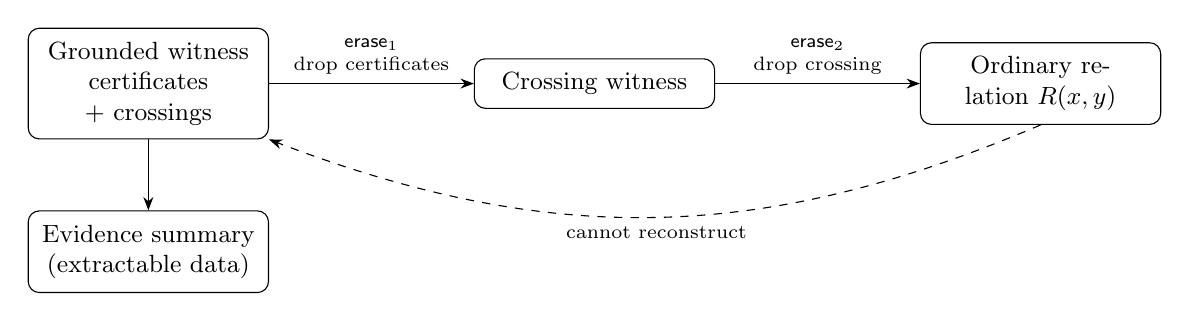
\begin{tikzpicture}[node distance=9mm and 26mm, box/.style={draw,rounded corners,align=center,inner sep=5pt,font=\small,text width=2.7cm}, lab/.style={align=center,font=\scriptsize}, >=Stealth]
\node[box] (G) {Grounded witness\\ certificates $+$ crossings};
\node[box,right=of G] (C) {Crossing witness};
\node[box,right=of C] (R) {Ordinary relation $R(x,y)$};
\node[box,below=of G] (S) {Evidence summary (extractable data)};
\draw[->] (G) -- node[above,lab]{$\erase_1$\\ drop certificates} (C);
\draw[->] (C) -- node[above,lab]{$\erase_2$\\ drop crossing} (R);
\draw[->] (G) -- (S);
\draw[->,dashed,bend left=22] (R.south) to node[below,lab]{cannot reconstruct} (G.south east);
\end{tikzpicture}
\caption{Two-stage erasure. The dashed arrow marks what erasure loses irreversibly (\cref{thm:nonreflect,thm:multiplicity}). The evidence summary is a separate, lossy projection that keeps extractable identifiers.}
\label{fig:erasure}
\end{figure}

\begin{table}[t]
\centering\small
\caption{Grounded versus ordinary rewriting.}\label{tab:compare}
\begin{tabularx}{\textwidth}{@{}lYY@{}}
\toprule
 & Ordinary rewriting & Grounded transport \\
\midrule
Judgement & $R(x,y) : \Prop$ & $\GTrans_c(x,y) : \Type$ \\
Inhabitants & Indistinguishable proofs & Distinguishable witnesses \\
Carries seam / lineage / coverage & No & Yes, as data \\
Contexts & $\Proper$: preserves the relation & $\GProper$: maps witnesses \\
Failure & Absence of proof & Located obstruction, or open obligation \\
Relation to the other & --- & Erases to it; not conversely \\
\bottomrule
\end{tabularx}
\end{table}

\subsection{Soundness and the erased preorder}
\begin{theorem}[Erasure soundness]\label{thm:sound}
If $w : \GTrans_c(x,y)$ then $R(x,y)$, where $R$ is agreement of the coordinate valuations. (\coq{erase_sound}, \coq{rpath_sound}; generically \coq{erasure_sound})
\end{theorem}
For a generic structure $G$ define the \emph{erased relation} $\mathsf{erased}_G(x,y) :\equiv \mathsf{inhabited}(\GTrans_G(x,y))$.
\begin{theorem}[Erased preorder]\label{thm:preorder}
$\mathsf{erased}_G$ is reflexive and transitive, and is contained in $R$. (\coq{erased_PreOrder}, \coq{erasure_sound})
\end{theorem}
Since composition holds up to $\weq$ (\cref{thm:algebra}) but the erased relation only records inhabitation, the erased relation satisfies the ordinary preorder laws with no qualification.

\subsection{Sound refinement versus exact recovery}
One must be careful with the word ``recovery''. If the erased relation \emph{is defined} as the image of grounded transport, then $R_G(x,y) \Longleftrightarrow \exists w : \GTrans(x,y)$ holds by definition. If instead one starts from an independently defined relation $R$, the general result is only the soundness map $\GTrans(x,y) \to R(x,y)$. The converse,
\[
R(x,y) \Longrightarrow \|\GTrans(x,y)\|,
\]
requires a completeness (representability) hypothesis $\mathsf{Complete}(G)$, under which $R$ and $\mathsf{erased}_G$ coincide (\coq{erasure_exact_of_complete}); it holds for the trivial structure whose witnesses are the proofs themselves (\coq{preorder_complete}). It fails in precisely the cases of interest. We therefore call the generic result a \emph{sound refinement}, not an equivalence with all ordinary rewriting.

\subsection{Non-reflection}
\begin{theorem}[Erasure does not reflect grounding]\label{thm:nonreflect}
There exist a transport problem $c$ and states $x,y$ with $R(x,y)$ and $\neg\,\mathsf{erased}(x,y)$. (\coq{erasure_not_reflecting}, \coq{copied_ungrounded_agreement})
\end{theorem}
\begin{proof}[Instance]
Take the dual-write problem of \cref{sec:example}, states $x = \mathsf{inl}(r_*)$ and $y = \mathsf{inr}(r_*)$. Both coordinate valuations are true, so $R(x,y)$. Every crossing requires a certified transport, and a certified transport would include the grounding equations at $r_*$, which fail; the declared lineage independently fails L1. So the problem admits no certified transport, and every witness is the identity path; since $x \neq y$, none connects them.
\end{proof}
The same fact is a generic \emph{ungrounded agreement}: extensional agreement without a transport witness, whose existence refutes $\mathsf{Complete}$ and hence exact recovery.

\subsection{Same endpoints, different warrants}
\begin{theorem}[Warrant multiplicity]\label{thm:multiplicity}
There exist $w_1, w_2 : \mathsf{PackedWarrant}(x,y)$ for the same endpoints such that both erase into $\mathsf{ErasedAt}(x,y)$, while their extractable summaries differ, and hence $w_1 \neq w_2$. (\coq{packed_warrants_same_endpoints}; within one problem \coq{same_endpoints_different_warrants})
\end{theorem}
The witnesses in our instance differ in seam element, exhibition record, custodian, coverage interval, authority, and---across problems---declared lineage dispositions. We do not assert equality of the two erased \emph{proofs}: $\mathsf{ErasedAt}$ is a proposition, so equality of its proofs would require proof irrelevance and would be uninformative. The content is that erasure maps both witnesses into one proposition that records nothing about which was used, while the summary separates them. This is the most direct proof that ordinary rewriting forgets evidential structure.

\section{Grounded-proper contexts}\label{sec:contexts}

\subsection{Definition}
A context $F : X \to Y$ is \emph{grounded-proper} between structures $G_X, G_Y$ when it maps witnesses functorially:
\[
\mathsf{map}_F : \GTrans_{G_X}(x,y) \to \GTrans_{G_Y}(Fx, Fy),
\]
with $\mathsf{map}_F(\mathsf{id}) = \mathsf{id}$ and $\mathsf{map}_F(v \circ w) = \mathsf{map}_F(v) \circ \mathsf{map}_F(w)$. This is stronger than $\Proper$, which maps only proofs of a relation: $\GProper$ preserves the \emph{warrant} for the relation. (\coq{GroundedProper})

\subsection{Identity and composition}
\begin{theorem}[Grounded-proper composition]\label{thm:gpcomp}
The identity context is grounded-proper, and if $F$ and $G$ are grounded-proper then so is $G \circ F$. (\coq{gp_id}, \coq{gp_comp}, \coq{grounded_proper_compose})
\end{theorem}

\subsection{Nested contextual preservation}
\begin{theorem}[Contextual preservation]\label{thm:ctx}
If $w : \GTrans(x,y)$ and $C_1,\dots,C_n$ are grounded-proper, then
\[
\mathsf{map}_{C_n}\cdots\mathsf{map}_{C_1}(w) : \GTrans\bigl(C_n[\cdots C_1[x]],\ C_n[\cdots C_1[y]]\bigr),
\]
and the witness map of a composite context is the composite of witness maps. (\coq{contextual_preservation}, \coq{contextual_preservation_nested})
\end{theorem}

\subsection{Erased \texttt{Proper}}
Every grounded-proper context induces an ordinary proper instance for the erased relation, $\Proper(\mathsf{erased}_{G_X} \Rightarrow \mathsf{erased}_{G_Y})\,F$ (\coq{grounded_proper_erased}, \coq{grounded_proper_Proper}). The converse is \emph{not} claimed: a context may preserve endpoint equivalence while discarding or fabricating lineage, so an ordinary $\Proper$ instance does not yield a witness map.

\subsection{Relation to rewriting tactics}
The development provides semantic combinators and instances, not an automated witness-carrying rewriting tactic. This separates the semantic kernel from later proof engineering: a tactic consuming the kernel should fail only when no suitable witness was supplied or constructed, never because the semantics needed weakening.

\section{Grounded seams as a canonical instance}\label{sec:seams}

\subsection{Spans, valuations and three-way grounding}
A span $A \xleftarrow{\back} \Sigma \xrightarrow{\fwd} B$ carries Boolean valuations $\Phi_A$, $\Phi_B$ and a seam valuation $\Phi_\Sigma$. The \emph{grounding equations} require both coordinate valuations to agree with the independently exhibited seam valuation:
\[
\Phi_A(\back(r)) = \Phi_\Sigma(r), \qquad \Phi_B(\fwd(r)) = \Phi_\Sigma(r) \qquad (r \in \Sigma).
\]
Contrast \emph{extensional seam agreement}, which is only pairwise: $\Phi_A(\back(r)) = \Phi_B(\fwd(r))$.

The definitions here are those of an earlier, separately published supplement, which we preserve byte-for-byte and build as an independent library (\cref{sec:mechanisation}). Our compatibility layer takes states to be $A + B$ and defines crossing witnesses as paths of crossings, where a crossing at $r$ carries \emph{both} grounding equations against $\Phi_\Sigma$. An earlier reconstruction of this instance used only the pairwise equation; it collapsed exactly the distinction this paper is about, and is retained only as a clearly labelled weaker layer.

\subsection{Grounding erases to extensional coherence}
\begin{theorem}[Grounding erases]\label{thm:ground-erases}
$\mathsf{GroundingEquations} \Longrightarrow \forall r,\ \Phi_A(\back(r)) = \Phi_B(\fwd(r))$. (\coq{original_grounding_erases_to_extensional})
\end{theorem}
The proof goes through the generic calculus: the equations supply a crossing at every seam element, and erasure yields pairwise agreement.

\subsection{Non-converse}
\begin{theorem}[Pairwise agreement does not imply grounding]\label{thm:pairwise}
There exist a span and valuations with pairwise agreement at every seam element but no grounding. (\coq{pairwise_agreement_not_grounding}; from \coq{copied_extensionally_coherent} and \coq{copied_not_grounded})
\end{theorem}
The witness is the dual-write example. Its generic reading is \cref{thm:nonreflect}: the legacy counterexample embeds as an instance of ungrounded agreement (\coq{original_copied_counterexample_embeds}), and, conversely, the legacy \coq{copied_not_grounded} is recovered from the generic obstruction (\coq{copied_not_grounded_from_generic}).

\subsection{Extensional factor transport}
We state the weak theorem first. Let $M_A : A \to O_A$ and suppose $\Phi_A = h \circ M_A$.
\begin{theorem}[Extensional factor transport]\label{thm:extfactor}
If extensional seam agreement holds, then $\Phi_B(\fwd(r)) = h(M_A(\back(r)))$ for every $r$. (\coq{extensional_factor_transport})
\end{theorem}

\subsection{Grounded factor transport}
\begin{corollary}[Grounded factor transport]\label{cor:groundedfactor}
If the grounding equations hold and $\Phi_A = h \circ M_A$, then $\Phi_B(\fwd(r)) = h(M_A(\back(r)))$. (\coq{grounded_factor_transport}; in exactly the legacy statement, \coq{original_seam_transport_from_generic})
\end{corollary}
The route is $\mathsf{GroundingEquations} \Rightarrow \mathsf{ExtensionalAgreement} \Rightarrow$ factor transport. Both theorems have the \emph{same conclusion}; the grounded one has stronger premises. The interpretation is the point of this paper in miniature:
\begin{quote}
\emph{Grounding does not change the endpoint equation. It changes the warrant carried with the use of that equation.}
\end{quote}
This is not a weakness to be hidden. The endpoint equation can remain true after the warrant supporting it has failed (\coq{extensional_conclusion_survives_ungrounded}); that is exactly what non-reflection expresses. A reviewer who observes that the earlier theorem uses stronger premises than its conclusion needs is correct, and the observation is part of the contribution.

\subsection{Compatibility}
The unchanged earlier supplement instantiates the generic calculus, and its transport theorem is recovered from it with the statement unchanged. This establishes continuity and makes clear which material is new: the generic calculus, erasure, contexts, obstruction, and assessment. The earlier supplement's files are checksum-verified in the build (\cref{sec:mechanisation}).

\section{Dynamic grounded transport}\label{sec:dynamic}

The synchronic grounding of \cref{sec:seams} concerns one stage. This section asks what survives when the system evolves. The answer separates four notions that are easily conflated: structural naturality, valuation naturality, preservation of grounding, and coverage.

\subsection{Structural seam evolution}
A seam evolution from stage $t$ to $u$ consists of maps $U^\Sigma_{t,u}$, $U^A_{t,u}$, $U^B_{t,u}$ on the seam and the two coordinates such that the squares commute:
\[
\back_u \circ U^\Sigma_{t,u} = U^A_{t,u} \circ \back_t, \qquad
\fwd_u \circ U^\Sigma_{t,u} = U^B_{t,u} \circ \fwd_t.
\]
Evolutions have identity and composition. We recover both from the earlier supplement, and show that the state map of a composite evolution agrees pointwise with the composite of state maps (\coq{evo_state_id}, \coq{evo_state_compose}), so the composite evolution and \coq{gp_comp} of the steps act identically.

\subsection{Structural versus valuational naturality}
The commuting squares say nothing about valuations. If the value spaces carry a transport $U^V_{t,u}$, one may additionally require all three valuations to be natural:
\[
\Phi_{A,u} \circ U^A_{t,u} = U^V_{t,u} \circ \Phi_{A,t}, \quad
\Phi_{B,u} \circ U^B_{t,u} = U^V_{t,u} \circ \Phi_{B,t}, \quad
\Phi_{\Sigma,u} \circ U^\Sigma_{t,u} = U^V_{t,u} \circ \Phi_{\Sigma,t}.
\]
We do not require the values to stay unchanged: a dynamic predicate may change while remaining coherently transported. Requiring $U^V = \mathrm{id}$ would turn a dynamic predicate into a temporal invariant.

\subsection{Preservation on the image}
Define $\mathsf{PreservesGroundingOnImage}(U)$: for every seam element $r$, grounding at $t$ implies grounding at $U^\Sigma_{t,u}(r)$. It concerns only seam elements \emph{of the form} $U^\Sigma_{t,u}(r)$, and says nothing about target elements outside the image.
\begin{theorem}[Naturality preserves grounding on the image]\label{thm:preserve}
If the structural squares commute and all three valuations are natural with respect to some $U^V$, then $\mathsf{PreservesGroundingOnImage}(U)$. In particular, if grounding holds at $t$ it holds at every transported seam element at $u$. (\coq{natural_valuations_preserve_grounding_on_image}, \coq{grounding_at_transported_elements})
\end{theorem}
Naturality also composes, with $U^V$ composing (\coq{natural_id}, \coq{natural_compose}). A $\mathsf{SeamEvolution}$ that preserves grounding on the image is a grounded-proper context (\coq{original_grounding_preserving_evolution_is_grounded_proper}); the hypothesis is exposed in the name because the witness map must send a grounded crossing at $r$ to a grounded crossing at its image.

\subsection{Coverage}
\begin{theorem}[Global preservation under coverage]\label{thm:coverage}
If $U^\Sigma_{t,u}$ is surjective, grounding is preserved on its image, and grounding holds throughout the seam at $t$, then grounding holds throughout the seam at $u$. (\coq{surjective_evolution_preserves_all_grounding})
\end{theorem}
Without surjectivity, new target seam elements require new grounding evidence. We exhibit a model in which preservation on the image holds and every stage-$t$ element is grounded, yet a new stage-$u$ element outside the image is not (\coq{preservation_without_coverage}). This separates \emph{continuation} from \emph{coverage}, and fits the intended reading: a new process requires a new certificate.

\begin{figure}[t]
\centering
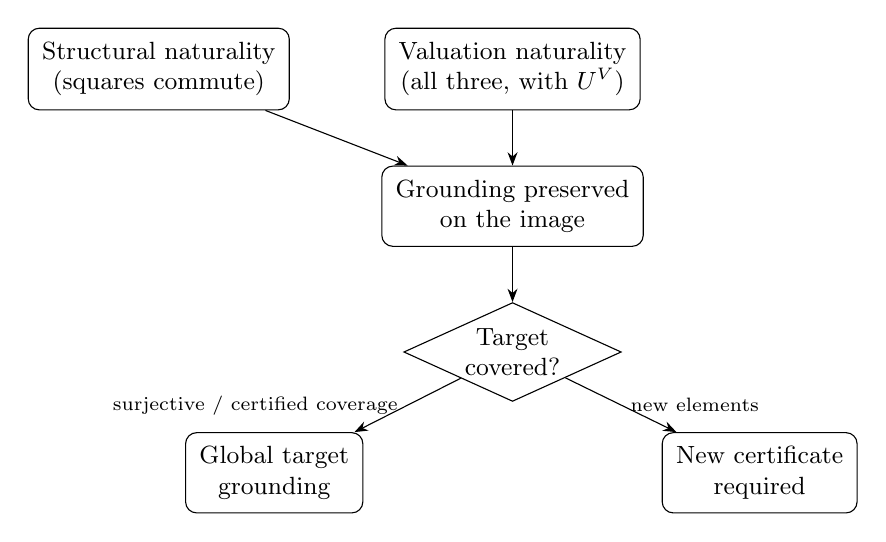
\begin{tikzpicture}[node distance=7mm and 12mm, box/.style={draw,rounded corners,align=center,inner sep=5pt,font=\small}, dia/.style={draw,diamond,aspect=2.2,align=center,inner sep=1pt,font=\small}, >=Stealth]
\node[box] (S) {Structural naturality\\ (squares commute)};
\node[box,right=of S] (V) {Valuation naturality\\ (all three, with $U^V$)};
\node[box,below=of V] (G) {Grounding preserved\\ on the image};
\node[dia,below=of G] (C) {Target\\ covered?};
\node[box,below left=of C] (A) {Global target\\ grounding};
\node[box,below right=of C] (N) {New certificate\\ required};
\draw[->] (S) -- (G);
\draw[->] (V) -- (G);
\draw[->] (G) -- (C);
\draw[->] (C) -- node[left,font=\scriptsize]{surjective / certified coverage} (A);
\draw[->] (C) -- node[right,font=\scriptsize]{new elements} (N);
\end{tikzpicture}
\caption{Structural and valuational preservation. Structure alone does not give preservation of grounding; preservation alone does not give coverage.}
\label{fig:dynamic}
\end{figure}

\subsection{Dynamic failure}
\begin{theorem}[Extensional persistence without grounded preservation]\label{thm:dynfail}
There is an evolution for which the structural squares commute; extensional agreement holds at both stages; grounding holds at $t$; and grounding fails at the transported element at $u$. Ordinary factor transport remains available at $u$. (\coq{dynamic_failure_visible}, \coq{ordinary_rewriting_still_succeeds}, \coq{structural_naturality_not_preservation})
\end{theorem}
The model has two stages and one seam element. The coordinates read true at both stages, so pairwise agreement persists. The seam valuation is true at the first stage and false at the second. No evolution preserves grounding, because the unique transported element loses it. This is the formal maintenance-debt example: warrant was valid at issuance, the system evolved, and the coordinates continue to agree while the independently evolved ground no longer does.

\subsection{Interpretive consequence}
Structural naturality preserves the relationship between carriers and projections. It does not, by itself, preserve the warrant attached to their valuations. A migration whose squares commute can be structurally faithful and evidentially stale.

\section{Obstructions to substitution}\label{sec:obstruction}

\subsection{Fibre obstruction}
Let $M : X \to O$ be an observation map and $\Phi : X \to V$ a predicate. $\Phi$ factors through $M$ iff it is constant on the fibres of $M$; this is the established factorisation criterion, a set-theoretic form of the Doob--Dynkin lemma and of the exactness condition of abstract interpretation \cite{cousot1977}, and we use it as such. A pair $x,y$ with $M(x) = M(y)$ and $\Phi(x) \neq \Phi(y)$ certifies that $\Phi$ cannot be determined from the observations alone (\coq{fibre_obstruction}). The direction from factorisation to fibre-constancy and the relational converse are constructive (\coq{factors_constant}, \coq{constant_relational}); the finite converse needs a complete enumeration and decidable equality (\coq{finite_constant_factors}); the unrestricted functional converse needs classical choice and is isolated (\cref{sec:mechanisation}).

\subsection{Lineage-sensitive obstruction}
\begin{theorem}[Observational agreement cannot license lineage-sensitive substitution]\label{thm:lineage-obs}
If $M(x) = M(y)$ and a predicate $L$ has $L(x) \neq L(y)$, then $\neg\,\Proper(\sim_M, =)(L)$. Moreover, if grounded transport is sound for agreement of $L$, then no transport witness connects $x$ and $y$. (\coq{not_proper_of_distinguished}, \coq{observational_insufficient}, \coq{observational_not_grounded})
\end{theorem}
The instance is the dual-write example: the copied value is identical on both requests, yet the exhibited trace status separates them, so the trace status is not determined by the copied value (\coq{trace_not_determined_by_copied_value}). The stronger, grounded reading is that observational equivalence $M(x) = M(y)$ does not imply $\GTrans(x,y)$.

\subsection{Located obstruction data}
Failures are represented as data that names the defect, not as a Boolean. The construction obligation can fail by: an empty seam; a seam element on which a coordinate valuation departs from the seam valuation; a defeated exhibition; a lineage descent (an ancestor path from a coordinate to the ground); an undisclosed shared ancestor (naming the node); the absence of an independent claim-relevant source; or a malformed lineage record. The observational obligation fails by a \emph{fibre witness} (a pair of states). The maintenance obligation, for temporal systems, fails by either the absence of any structural evolution or, for every evolution, a named seam element at which grounding is lost. Authority failure is a type supplied by the application.

Each located failure comes with a proof that it refutes the corresponding evidence, so a failure is not merely a label but a counter-argument (\coq{located_refutes}).

\subsection{Obstruction versus absence of evidence}
A located obstruction warrants rejection. A missing record may instead leave the assessment open. A missing lineage record, a lineage record with declared coverage gaps, and an incomplete finite search are all \emph{unresolved}, not refuted; only a proved defect refutes. Keeping these apart is what allows the assessment of \cref{sec:assessment} to avoid collapsing three different situations into one negative answer.

\section{Evidence-bearing transport assessment}\label{sec:assessment}

\subsection{Component verdicts}
For each obligation an assessment is one of three things: a positive certificate, located counterevidence, or an identification of what is missing.
\[
\Assess(P) \;=\; \mathsf{Discharged}(e) \;+\; \mathsf{Failed}(d) \;+\; \mathsf{Unresolved}(o),
\]
where $e$ is positive evidence, $d$ is located counterevidence, and $o$ names the missing evidence or decision. In the development, unresolved reasons include a not-yet-assessed obligation, a missing lineage record, a coverage gap (naming the gaps), an incomplete search, and an undeclared policy.

\subsection{Four diagnostic loci}
The obligations instantiate four loci: \emph{observation} (the valuation factors through the observations), \emph{construction} (an exhibited seam with independently grounded lineage), \emph{maintenance} (warrant preserved through evolution), and \emph{institution} (a declared rule or authority licenses the transformation). They are diagnostic loci, not a partition: failures can coexist.

\subsection{The assessment type}
For a transport problem $c$,
\begin{lstlisting}
Inductive TransportAssessment (c : EvCandidate) : Type :=
| Certified : CertifiedTransport c -> TransportAssessment c
| Refuted   : Obstructions c        -> TransportAssessment c   (* head :: tail *)
| Open      : list OpenObligation   -> TransportAssessment c.
\end{lstlisting}
$\Cert(w)$ carries the evidence warranting transport; $\Refu(os)$ carries a \emph{non-empty} collection of located obstructions; $\Open(ds)$ names the unresolved obligations. The assembly function combines the four component verdicts.

\begin{figure}[t]
\centering
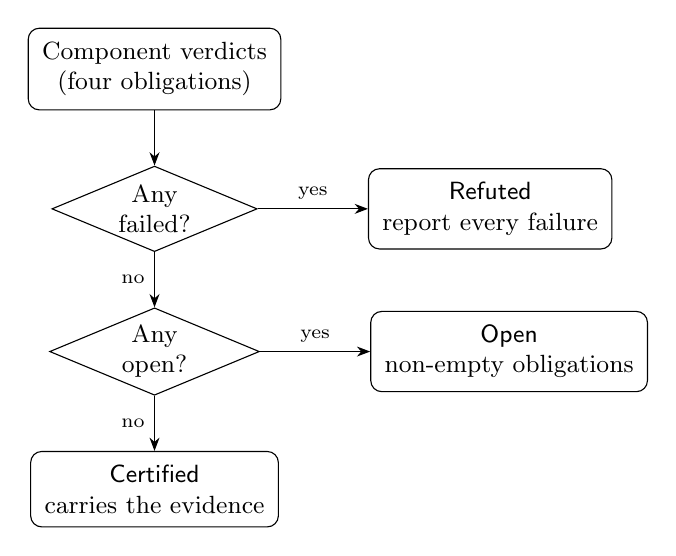
\begin{tikzpicture}[node distance=7mm and 14mm, box/.style={draw,rounded corners,align=center,inner sep=5pt,font=\small}, dia/.style={draw,diamond,aspect=2.4,align=center,inner sep=1pt,font=\small}, >=Stealth]
\node[box] (A) {Component verdicts\\ (four obligations)};
\node[dia,below=of A] (F) {Any\\ failed?};
\node[box,right=of F] (R) {\textsf{Refuted}\\ report every failure};
\node[dia,below=of F] (O) {Any\\ open?};
\node[box,right=of O] (U) {\textsf{Open}\\ non-empty obligations};
\node[box,below=of O] (C) {\textsf{Certified}\\ carries the evidence};
\draw[->] (A) -- (F);
\draw[->] (F) -- node[above,font=\scriptsize]{yes} (R);
\draw[->] (F) -- node[left,font=\scriptsize]{no} (O);
\draw[->] (O) -- node[above,font=\scriptsize]{yes} (U);
\draw[->] (O) -- node[left,font=\scriptsize]{no} (C);
\end{tikzpicture}
\caption{Verdict aggregation. Verdicts are singular; the \emph{report} behind a verdict retains every failed and every open obligation (\cref{thm:report}).}
\label{fig:aggregation}
\end{figure}

\subsection{Reports versus verdicts}
The aggregate verdict and the complete report are different things and we keep them apart. The verdict follows the componentwise rule: no failure and no open obligation gives $\Cert$; at least one failure gives $\Refu$; no failure but at least one open obligation gives $\Open$ (\coq{assemble_status}). The \emph{report} lists every obligation in exactly one of three lists---failed, open, discharged---whatever the verdict.
\begin{theorem}[Complete reporting]\label{thm:report}
The verdict of the report is the verdict of the assembled assessment, and every obligation is accounted for exactly once: $|\text{failed}| + |\text{open}| + |\text{discharged}| = 4$. (\coq{report_verdict_agrees}, \coq{report_accounts_for_all})
\end{theorem}
The distinction matters. The $\Refu$ constructor itself carries the located failures; if a failure co-occurs with an unresolved obligation, the verdict is $\Refu$ but the open obligation must not vanish because another obligation already refutes transport. It does not: it remains in the report (\coq{refuted_verdict_keeps_open_item}, where a copied ground fails construction while maintenance is unassessed). This was a gap in an earlier form of the development, in which the assembled $\Refu$ value dropped co-occurring open items; it is repaired by separating the report from the verdict.

\subsection{Soundness and characterisation}
\begin{theorem}[Certification soundness]\label{thm:certsound}
A certified assessment carries certified transport, and that erases to the legacy $\mathsf{Transportable}$ predicate. An assembled assessment is $\Cert$ exactly when every obligation is discharged. (\coq{certified_gives_transportable}, \coq{assemble_status})
\end{theorem}
\begin{theorem}[Refutation soundness]\label{thm:refsound}
If $o$ is a collection of located obstructions for $c$, no certified transport for $c$ exists, and this holds of \emph{every} member of the collection. (\coq{obstructions_refute}, \coq{each_obstruction_refutes})
\end{theorem}
\begin{theorem}[Open transport]\label{thm:open}
An assembled assessment is $\Open$ iff no obligation has located counterevidence and at least one obligation is unresolved; it neither asserts transportability nor its negation. Moreover an $\Open$ assessment always names at least one unresolved obligation. (\coq{assemble_status}, \coq{underdetermined_iff}, \coq{assemble_open_nonempty})
\end{theorem}
\begin{theorem}[Complete failure reporting]\label{thm:allfail}
A refuted assembly reports \emph{every} failed obligation, in a fixed order (observational, construction, maintenance, institutional). (\coq{assemble_refuted_reports_all})
\end{theorem}
Thus assessment is \emph{cumulative} rather than precedence-based: in a model where a copied ground and a lost grounding coexist, both obstructions appear (\coq{both_obstructions_reported}). Verdicts may be singular, but warrant failures are cumulative.

\subsection{Decidable specialisation}
When every obligation has a decision procedure the open case disappears: the status is then never $\Open$, and $\Cert$ (resp.\ $\Refu$) coincides with transport (resp.\ its negation) for the conjunction of the obligations (\coq{decidable_not_underdetermined}, \coq{decided_certified_iff_transport}, \coq{decided_refuted_iff_not_transport}). A Boolean classifier is thereby a \emph{specialisation} of the evidence-sensitive assessment, not its foundation. General admissibility, institutional adequacy, and real-world lineage completeness are not assumed decidable. The manuscript-level status ``warrant conflict'' cannot arise here, since one assessment of one obligation is exactly one of the three cases.

\section{Finite lineage certificates}\label{sec:lineage}

\subsection{Data model}
A \emph{lineage record} is finite data: the derived fields with their parents; the raw inputs; the claim-relevant raw inputs; three distinguished nodes $d_A$, $d_B$ and $g$ (the determinations $\Phi_A \circ \back$, $\Phi_B \circ \fwd$ and $\Phi_\Sigma$); and a disposition (justified, or open defeater) for shared ancestors. It is represented as lists of numbers so that it survives extraction.

\subsection{Lineage conditions}
Write $\anc(x)$ for the strict ancestors of $x$. The valuation $\Phi_\Sigma$ is \emph{lineage-grounded} when:
\begin{description}
\item[L1, no descent:] $d_A \notin \anc(g)$ and $d_B \notin \anc(g)$;
\item[L2, disclosure:] every shared non-raw ancestor of $d_A$ and $d_B$ carries a disposition;
\item[L3, independent source:] the ground-only ancestry contains a claim-relevant raw input.
\end{description}
Well-formedness is part of the requirement: unique names, declared parents, distinguished nodes derived, relevant inputs raw, and acyclicity.

\subsection{Coverage}
A passing verdict applies only to the declared graph \emph{and} its declared coverage. A partial graph must not be reported as globally lineage-grounded; the record carries its declared gaps, and a passing graph with non-empty gaps is coverage-qualified, hence open, not accepted.

\subsection{A checked decision procedure}
We define the audit as a function $\mathsf{lineageCheck}(g,c)$ over a lineage record $g$ and coverage record $c$, returning \emph{accepted}, \emph{rejected with a located defect}, or \emph{open with the gaps}. Ancestors are computed by iterating a de-duplicating closure step as many times as there are nodes; the correctness argument is a pigeonhole one and needs only that every parent is a declared node.
\begin{theorem}[Ancestor correctness]\label{thm:anc}
$\mathsf{ancestors}$ is sound, and complete when parents are declared: $m \in \mathsf{ancestors}(n) \Longleftrightarrow$ $m$ is a strict ancestor of $n$. (\coq{ancestors_sound}, \coq{ancestors_complete}, \coq{ancestors_iff})
\end{theorem}
\begin{theorem}[Lineage-check reflection]\label{thm:reflect}
Unconditionally,
\[
\mathsf{lineageCheck}(g,c) = \mathsf{Accepted} \;\Longleftrightarrow\; \mathsf{LineagePasses}(g) \wedge \mathsf{gaps}(c) = [\,].
\]
A rejection is located and its evidence is proved; an open result means exactly that the graph passes while gaps remain. (\coq{lineage_check_reflect}, \coq{defect_sound}, \coq{lineage_check_rejected}, \coq{lineage_check_open})
\end{theorem}
Reflection is unconditional, without a well-formedness hypothesis, because well-formedness is itself checked and reflected: soundness and completeness of ancestors are needed to reflect acyclicity. Each of well-formedness, L1, L2 and L3 is separately reflected (\coq{wf_defect_none_iff}, \coq{check_L1_reflect}, \coq{undisclosed_none_iff}, \coq{check_L3_reflect}). An accepted check constructs a kernel-checked certificate whose graph and coverage are the ones checked (\coq{issue_certificate_iff}, \coq{issue_certificate_data}), and a rejection converts to a located construction failure for assessment.

\subsection{The audit boundary}
It is important to state exactly what is and is not proved. The Coq predicate and the Coq checker are related by \cref{thm:reflect}. The \emph{handwritten} OCaml audit that accompanies the case study is \emph{not} proved equivalent to either; it implements the same stated conditions, and its agreement with the checked procedure is established by regression testing (\cref{sec:evaluation}), not by a theorem.

The extracted checker can take over the decision core: the handwritten code remains as input construction, diagnostic formatting, the case-study driver, and an independent comparison. This is preferable to verifying arbitrary handwritten OCaml against Coq after the fact. We have not yet replaced the handwritten decision core in the supplement, whose files are preserved unchanged.

\section{Mechanisation and executable evidence}\label{sec:mechanisation}

\subsection{Development structure}
The development comprises roughly three thousand lines of theory and eight hundred of examples. Its layers are kept separate:
\begin{enumerate}
\item the \textbf{legacy layer}: an earlier supplement, imported byte-for-byte, checksum-verified, and built as an independent library;
\item the \textbf{generic calculus}: the kernel structure, erasure, grounded-proper contexts, and obstructions;
\item the \textbf{compatibility layer}: proofs that the legacy seam, evolution and admissibility definitions instantiate the generic ones;
\item the \textbf{assessment layer}: certificates, witnesses, located obstructions, assessments, the lineage checker, packed warrants;
\item \textbf{examples}: the separating models of \cref{sec:evaluation}.
\end{enumerate}
The generic calculus is not replaced by the legacy material; each is preserved, and the compatibility layer proves that the original definitions instantiate the generic ones.

\subsection{Trust boundary}
\begin{table}[t]
\centering\small
\caption{Trust boundary and non-claims.}\label{tab:trust}
\begin{tabularx}{\textwidth}{@{}lY@{}}
\toprule
Checked mechanically & Coq 8.18.0; build with \texttt{coq\_makefile} and \texttt{dune}; \texttt{coqchk} on the whole project except the isolated classical file; \texttt{Print Assumptions} for every reported theorem; checksum verification of the legacy supplement. \\
Trusted & The Coq kernel and extraction mechanism; the encoding of $\nat$ as OCaml integers in extracted code; the declared records themselves. \\
Not established & Completeness of declared lineage; accuracy of raw inputs; adequacy of the state model; legitimacy or competence of an authority; decidability of general obligations; equivalence of the handwritten OCaml audit with the checked one. \\
\bottomrule
\end{tabularx}
\end{table}

\subsection{Classical factorisation}
The unrestricted functional converse of fibre factorisation needs classical choice and is isolated in one file that nothing else imports; the rest of the development is axiom-free. The constructive alternatives are the relational formulation and the finite theorem with a complete enumeration and decidable equality. The main development does not depend on the classical file: \texttt{coqchk} succeeds on the project without it and reports no axioms.

\subsection{Extraction behaviour}
Certificate data live in \texttt{Type}; their proofs live beside them. Extraction removes the proof fields and keeps the data.

\begin{table}[t]
\centering\small
\caption{Evidence fields and whether they survive extraction.}\label{tab:survive}
\begin{tabularx}{\textwidth}{@{}lYc@{}}
\toprule
Component & Field & Survives \\
\midrule
Exhibition certificate & record id, identifiers, process, retained record and evaluator, coverage, custodian & yes \\
 & injectivity of identifiers; valuation factorisation proof & no \\
Lineage certificate & graph, coverage record with gaps, issued verdict & yes \\
 & well-formedness, L1--L3 proofs & no \\
Construction certificate & seam inhabitant & yes \\
 & grounding equations & no \\
Obstruction & constructor tag; located data (seam element, node id) & yes \\
 & Prop-valued evidence & no \\
Assessment & verdict, open reasons, gaps & yes \\
Maintenance / authority & application-supplied data, via the summary interface & if in \texttt{Type} \\
\bottomrule
\end{tabularx}
\end{table}

We extracted the assessments of the examples to OCaml and wrote a consumer. For a certified assessment it reports the custodian (7), record id (1), lineage ground node (5) and audit verdict (\texttt{LineagePass}). For the copied model it reports a refutation at construction whose constructor names a lineage descent; for the maintenance model, a maintenance obstruction; for the model with both, both, in order. This is the concrete content of the claim that the formal distinction survives compilation. It is materially stronger than attaching abstract propositions \texttt{Exhibited} and \texttt{LineageGrounded} to an ordinary relation, whose proofs would be erased.

\subsection{Evidence summaries}
Maintenance and authority evidence stay abstract in the generic library: the calculus should not impose one institutional record format. What it provides is a \emph{summary interface},
\begin{lstlisting}
Class EvidenceSummary (A : Type) := { evidence_summary : A -> list EvidenceAtom }.
\end{lstlisting}
with atoms for records, custodians, ground nodes, intervals, authorities, maintenance events, expiry and revalidation. Applications supply instances, so an extracted consumer can inspect more than the exhibition and lineage components without the kernel fixing a schema. This is an observability extension, not a kernel correctness gap; the witness summary now includes maintenance and authority atoms.

\section{Evaluation through separating examples}\label{sec:evaluation}

The examples are \emph{separating models}, not empirical evaluation: each is a small finite structure that shows a distinction is real. They establish that the formal separations hold; they do not establish usability or scalability on production systems.

\subsection{RQ1: Can ordinary agreement survive while grounding fails?}
\emph{Copied coordinates.} Extensional agreement succeeds and erasure yields ordinary substitutability; grounding fails at $r_*$; assessment is $\Refu$ with a construction obstruction (the declared lineage descends from a coordinate; independently, grounding fails at $r_*$). Ordinary agreement survives while grounded warrant fails (\cref{thm:nonreflect,thm:pairwise}).

\subsection{RQ2: Can structural naturality preserve agreement while losing grounding?}
\emph{Maintenance failure.} The squares commute; pairwise agreement persists at both stages and ordinary rewriting succeeds; grounding is lost at the transported element; assessment is $\Refu$ with a maintenance obstruction naming the seam element (\cref{thm:dynfail}). The same problem with maintenance unassessed is $\Open$, and with grounded valuations it is $\Cert$: one problem, three outcomes.

\subsection{RQ3: Can several failures be retained simultaneously?}
\emph{Co-occurrence.} A copied ground together with a lost grounding fails two obligations; both obstructions are reported, in a fixed order, with no first-error precedence discarding the second (\cref{thm:allfail}). A further variant fails one obligation and leaves another open: the verdict is $\Refu$ and the open obligation remains in the report (\cref{thm:report}).

\subsection{RQ4: Can different warrants erase to the same judgement?}
\emph{Different warrants.} Two witnesses, one within a single problem and one across problems with different declared lineage, connect the same endpoints and erase into the same judgement, while their summaries differ in record, custodian, coverage, authority, and lineage disposition (\cref{thm:multiplicity}).

\subsection{RQ5: Does missing evidence remain distinct from counterevidence?}
A missing lineage record yields $\Open$; a partial lineage record with declared gaps yields $\Open$ (coverage-qualified, under our declared standard); an explicit invalid lineage path yields $\Refu$. The checked audit distinguishes the last two on the same inputs: a passing graph with gaps is open, and a defect beats a gap.

\begin{table}[t]
\centering\small
\caption{Separating examples and outcomes.}\label{tab:examples}
\begin{tabularx}{\textwidth}{@{}lccY@{}}
\toprule
Example & Ordinary relation & Assessment & Located evidence \\
\midrule
Valid seam & holds & $\Cert$ & full witness: custodian, record, ground node, verdict \\
Copied coordinates & holds & $\Refu$ & lineage descent; grounding failure at $r_*$ \\
Missing lineage record & may hold & $\Open$ & \textit{missing lineage record} \\
Partial lineage record & may hold & $\Open$ & \textit{coverage gap}, gaps named \\
Dynamic failure & holds & $\Refu$ & lost grounding at transported element \\
Co-occurrence & holds & $\Refu$ & construction \emph{and} maintenance obstruction \\
Failure $+$ open & holds & $\Refu$ & failure reported; open item retained in report \\
\bottomrule
\end{tabularx}
\end{table}

\subsection{Lineage audit: regression against the handwritten audit}
The extracted, checked lineage procedure was compared with the handwritten OCaml audit of the case study, by capturing the latter's printed output. On the five case-study records (live rows; backfill with a disclosed shared ancestor; backfill with the shared ancestor undisclosed; a copied seam valuation; a cyclic record) the two agree on all five, including the malformed cycle. On 3000 randomly generated records, including every malformation kind (duplicate names, undeclared parents, distinguished nodes not derived, relevant inputs not raw, and cycles), the two agree on all 3000. The generated records were 89 grounded, 1403 not grounded, and 1508 malformed.

Two remarks. First, this is a \emph{test}: agreement on these inputs, not equivalence. Second, the harness discriminates. A deliberate mutation of the extracted side---dropping the $d_B$ descent test from L1---was detected by the random test and not by the five case-study records; the case study alone would not have found that fault. The accepting path is exercised less than the rejecting paths, since few random records are grounded.

\section{Relationship to existing formalisms}\label{sec:related}

\paragraph{Equality and setoid rewriting.}
Ordinary rewriting identifies the relation that contexts must respect; generalised rewriting in type theory makes this systematic with respectful morphisms \cite{sozeau2009}. Grounded transport additionally retains the evidence that licenses the relation in the particular case.

\paragraph{\texttt{Proper} and respectful morphisms.}
$\GProper$ refines $\Proper$: it maps witnesses, not merely the truth of a relation. Erasure turns grounded-proper contexts into ordinary proper contexts (\cref{sec:contexts}); the converse fails.

\paragraph{Proof-relevant relations.}
The calculus belongs to the family of proof-relevant relational structures, but adds application-specific certificate and assessment layers oriented towards lineage, maintenance and audit.

\paragraph{Rewriting logic and labelled transitions.}
Rewriting logic \cite{meseguer1992} and labelled transition systems retain transition labels. A label alone need not contain independently checkable lineage, coverage and warrant evidence. Grounded witnesses can be read as richly certified transition labels; we do not develop this reading formally here.

\paragraph{Categorical transport.}
Identity, composition and structure-preserving erasure suggest a categorical interpretation \cite{maclane1998}. We claim a category only up to the witness equivalence $\weq$ of \cref{sec:laws}, for which the laws are proved; a stronger claim would require witness equality we do not have.

\paragraph{Proof-carrying systems and certified transformations.}
Grounded transport resembles proof-carrying code \cite{necula1997} and certified compilation \cite{leroy2009} in carrying evidence across a transformation. Its distinctive concern is that the evidence includes grounding, lineage, open obligations and institutional parameters, not only semantic preservation.

\paragraph{Provenance systems.}
Provenance systems record derivational histories \cite{buneman2001,cheney2009}. Grounded transport adds claim-relative conditions determining whether that history licenses substitution: a history is not thereby a warrant.

\paragraph{Assurance cases.}
The certified/refuted/open distinction supports assurance cases that must retain defeaters and unresolved obligations rather than issue only success or failure \cite{bloomfield2020}.

\paragraph{Processual motivation.}
The settled endpoints correspond to coordinate description; the witness-bearing transition retains something of the production of that agreement \cite{whitehead1929}. The formal calculus does not encode any ontology and should not be read as doing so. It formalises one methodological consequence: endpoint agreement does not exhaust the conditions under which a processual transition warrants substitution. The full treatment, including the taxonomy of warrant debt, is in a companion manuscript \cite{companion}.

\begin{table}[t]
\centering\small
\caption{Comparison with related formalisms.}\label{tab:related}
\begin{tabularx}{\textwidth}{@{}lYY@{}}
\toprule
Formalism & Retains & Does not retain (in general) \\
\midrule
Setoid rewriting & the relation, context respect & how the relation was established \\
Rewriting logic / LTS & transition labels & checkable lineage, coverage, warrant \\
Proof-carrying code & semantic-preservation evidence & grounding independence, open obligations \\
Provenance & derivational history & when history licenses substitution \\
Assurance cases & arguments, defeaters & mechanised located obstructions \\
Grounded transport & seam, lineage, coverage, authority evidence; located failures; open items & real-world adequacy of declared records \\
\bottomrule
\end{tabularx}
\end{table}

\section{Limitations}\label{sec:limitations}

\paragraph{Declared-graph limitation.}
A lineage certificate proves properties of the \emph{declared} graph. It does not prove that the graph contains every real production path, and the audit cannot detect a production path the record omits.

\paragraph{Raw-input limitation.}
The calculus can identify claim-relevant raw inputs without proving that they accurately record the concrete process.

\paragraph{Institutional limitation.}
Authority and custodianship can be represented as data, but their legitimacy and competence are not established internally; the rule system is an input. Exhibition conditions concerning the declared process, coverage and custodian are recorded, not verified.

\paragraph{Decidability limitation.}
General transport obligations need not be decidable. The open assessment is essential, not an implementation inconvenience.

\paragraph{Coverage limitation.}
Preservation on the image of an evolution does not certify new target states outside that image (\cref{thm:coverage}).

\paragraph{The endpoint theorem is extensional.}
The equality concluded by seam transport needs only extensional agreement. Grounding strengthens its warrant, not its algebraic conclusion (\cref{sec:seams}).

\paragraph{Composition in the concrete instance.}
In a single seam a non-identity witness is one crossing, so composition of non-trivial witnesses is degenerate there; its content appears through contexts and evolution.

\paragraph{Witness algebra modulo an equivalence.}
Identity and associativity hold up to the crossing-sequence equivalence, not by literal equality (\cref{sec:laws}).

\paragraph{The audit boundary.}
The Coq checker is proved to reflect its specification; the handwritten OCaml audit is tested against it, not proved equivalent (\cref{sec:lineage,sec:evaluation}). The decision core of the supplement has not yet been replaced by the extracted checker. Assessment components for maintenance and authority are abstract in the generic library.

\paragraph{Boolean valuations.}
Valuations are Boolean; a general value space with a value transport is used only in the statement of valuation naturality.

\paragraph{No automated tactic yet.}
The contribution is semantic and mechanised, not a packaged rewriting tactic.

\paragraph{No empirical claim.}
The examples demonstrate logical separations, not usability or scalability on production systems.

\section{Conclusion}\label{sec:conclusion}

The central distinction is between
\[
\text{same endpoint judgement} \;\neq\; \text{same warrant}.
\]
Grounded transport carries evidence; composition and grounded-proper contexts preserve it; erasure yields ordinary substitutability and loses information irreversibly; located obstructions explain failed transport; open assessments preserve unresolved obligations, and a refutation does not discard them; and extraction retains the evidential data that downstream audits require.

Ordinary rewriting answers whether one expression may replace another under a relation. Grounded transport additionally answers through which process, under which lineage, within what coverage, and with which remaining obligations that replacement is warranted. Erasure recovers ordinary substitutability, but ordinary substitutability cannot reconstruct the warrant that was erased.

The calculus does not make declarations true. It makes precisely explicit what has been declared, checks what can be checked, and reports what has not been resolved.


\bibliographystyle{plainnat}
\bibliography{refs}

\appendix
\section{Theorem ledger}\label{app:ledger}

The main text is organised around the following theorem spine. Each row names the Coq identifier(s) in the accompanying development; helper lemmas are in the supplement. All listed results are closed under the global context (no axioms), except where noted.

{\small
\begin{longtable}{@{}r>{\raggedright\arraybackslash}p{4.6cm}>{\raggedright\arraybackslash}p{6.4cm}l@{}}
\caption{Theorem spine and its mechanisation.}\label{tab:ledger}\\
\toprule
\# & Result & Coq identifier(s) & Text \\
\midrule
\endfirsthead
\toprule
\# & Result & Coq identifier(s) & Text \\
\midrule
\endhead
\bottomrule
\endfoot
T1 & Grounded reflexivity & \coq{grounded_transport_refl} & \cref{thm:refl} \\
T2 & Grounded composition & \coq{grounded_transport_compose} & \cref{thm:compose} \\
T2$'$ & Witness algebra modulo $\weq$ & \coq{WEquiv_id_left}, \coq{WEquiv_id_right}, \coq{WEquiv_assoc}, \coq{WEquiv_compose} & \cref{thm:algebra} \\
T3 & Erasure soundness & \coq{erase_sound}, \coq{rpath_sound}, \coq{erasure_sound} & \cref{thm:sound} \\
T4 & Erased preorder & \coq{erased_PreOrder} & \cref{thm:preorder} \\
T5 & Erasure non-reflection & \coq{erasure_not_reflecting}, \coq{copied_ungrounded_agreement} & \cref{thm:nonreflect} \\
T6 & Same endpoints, different warrants & \coq{same_endpoints_different_warrants}, \coq{packed_warrants_same_endpoints} & \cref{thm:multiplicity} \\
T7 & Grounded-proper composition & \coq{gp_id}, \coq{gp_comp} & \cref{thm:gpcomp} \\
T8 & Nested contextual preservation & \coq{contextual_preservation_nested} & \cref{thm:ctx} \\
T9 & Grounding erases to extensional agreement & \coq{original_grounding_erases_to_extensional} & \cref{thm:ground-erases} \\
T10 & Pairwise agreement $\not\Rightarrow$ grounding & \coq{pairwise_agreement_not_grounding} & \cref{thm:pairwise} \\
T11 & Original seam transport recovered & \coq{original_seam_transport_from_generic} & \cref{cor:groundedfactor} \\
T12 & Naturality preserves grounding on the image & \coq{natural_valuations_preserve_grounding_on_image} & \cref{thm:preserve} \\
T13 & Global preservation under coverage & \coq{surjective_evolution_preserves_all_grounding} & \cref{thm:coverage} \\
T14 & Extensional persistence, grounding loss & \coq{dynamic_failure_visible} & \cref{thm:dynfail} \\
T15 & Lineage-sensitive obstruction & \coq{not_proper_of_distinguished}, \coq{observational_not_grounded} & \cref{thm:lineage-obs} \\
T16 & Certification soundness & \coq{certified_gives_transportable}, \coq{assemble_status} & \cref{thm:certsound} \\
T17 & Refutation soundness & \coq{obstructions_refute}, \coq{each_obstruction_refutes} & \cref{thm:refsound} \\
T18 & Open-status characterisation & \coq{assemble_status}, \coq{underdetermined_iff}, \coq{assemble_open_nonempty} & \cref{thm:open} \\
T19 & Complete failure reporting & \coq{assemble_refuted_reports_all}, \coq{report_accounts_for_all}, \coq{report_verdict_agrees} & \cref{thm:allfail,thm:report} \\
T20 & Lineage-check reflection & \coq{lineage_check_reflect}, \coq{ancestors_iff} & \cref{thm:reflect,thm:anc} \\
\midrule
--- & Functional converse of fibre factorisation (classical) & \coq{constant_factors} (isolated file) & \cref{sec:obstruction} \\
\end{longtable}
}

\paragraph{Supplement contents.}
Complete Coq listings; the \texttt{Print Assumptions} transcripts; the legacy checksum tables; build configuration; the extracted OCaml output and its consumers; and the regression harness for the lineage audit. The tactic implementation is not included, as none exists yet.


\end{document}
